\documentclass{article}
%\usepackage[francais]{babel}
%\usepackage[utf8]{inputenc} % Required for including letters with accents
%\usepackage[T1]{fontenc} % Use 8-bit encoding that has 256 glyphs
\usepackage{pythontex}
\usepackage{amsthm}
\usepackage{amsmath}
\usepackage{amssymb}
\usepackage{mathrsfs}
\usepackage{graphicx}
\usepackage{geometry}
\usepackage{stmaryrd}
\usepackage{tikz}
\usetikzlibrary{patterns}
%\usetikzlibrary{intersections}
\usepackage[cache=false]{minted}
\usepackage{xcolor}

\usepackage{stmaryrd}
%\usetikzlibrary{tikzmark}
\usepackage{empheq}
\usepackage{longtable}
\usepackage{booktabs} 
\usepackage{array}
\usepackage{pstricks}
\usepackage{pst-3dplot}
\usepackage{pst-tree}
\usepackage{pstricks-add}
\usepackage{upgreek}
%\usepackage{epstopdf}
\usepackage{eolgrab}
\usepackage{chngpage}
 \usepackage{calrsfs}
 % Appel du package pythontex 
\usepackage{pythontex}

\usepackage{algorithm2e}
\RestyleAlgo{algoruled}
  \SetKw{KwFrom}{from} 
\newenvironment{algo}{
\begin{algorithm}[H]
\DontPrintSemicolon \SetAlgoVlined}
{\end{algorithm}}



\usetikzlibrary{decorations.pathmorphing}
\def \de {{\rm d}}
\usepackage{color}
\usepackage{xcolor}
\newcommand{\mybox}[1]{\fbox{$\displaystyle#1$}}
\newcommand{\myredbox}[1]{\fcolorbox{red}{white}{$\displaystyle#1$}}
\newcommand{\mydoublebox}[1]{\fbox{\fbox{$\displaystyle#1$}}}
\newcommand{\myreddoublebox}[1]{\fcolorbox{red}{white}{\fcolorbox{red}{white}{$\displaystyle#1$}}}

\usepackage{xcolor}
%\setbeamercolor{background canvas}{bg=lightgray}
\definecolor{LightGray}{gray}{0.9}
\definecolor{monOrange}{rgb}{0.97,0.35,0.04}
\usepackage{enumitem}
 \title{Projet Boutique - partie 1}
\author{Ibrahim ALAME}
\date{14/02/2023}
\begin{document}
\maketitle

\section{Initialisation du projet}
\subsection{Initialisation du projet}
Placez-vous où vous voulez pour créer le nouveau projet en ouvrant un terminal. Par exemple dans HOME :
\begin{minted}[
mathescape,
framesep=2mm,
baselinestretch=1.2,
%fontsize=\footnotesize,
bgcolor=LightGray,
%linenos
]{bash}
cd
\end{minted}
Créez un nouveau projet {\color{monOrange}Vue.js} :
\begin{minted}[
mathescape,
framesep=2mm,
baselinestretch=1.2,
%fontsize=\footnotesize,
bgcolor=LightGray,
%linenos
]{bash}
npm init vue@latest
\end{minted}
\begin{enumerate}
\item Par défaut, le nom est prérempli avec {\color{monOrange}vue-project} mais vous pouvez bien sûr le changer par exemple par {\color{monOrange}boutique}.
\item  La deuxième question est sur l'utilisation de {\color{monOrange}TypeScript} :
\begin{minted}[
mathescape,
framesep=2mm,
baselinestretch=1.2,
%fontsize=\footnotesize,
bgcolor=LightGray,
%linenos
]{html}
Add TypeScript? … No / Yes
\end{minted}
Comme nous l'avons vu, choisissez oui.
\item Ensuite répondez non pour JSX. Nous n'utiliserons par JSX qui est un langage de {\color{monOrange}template React}.
\item Répondez non pour {\color{monOrange}Vue Router, Pinia, Vitest} et {\color{monOrange}Cypress} car nous les verrons plus tard dans la formation.
\item Répondez oui à {\color{monOrange}ESLint}, qui permet de contrôler la qualité du code et répondez oui à {\color{monOrange}Prettier} pour le formatage du code.
\end{enumerate}

Vous devez en être là :
\begin{center}
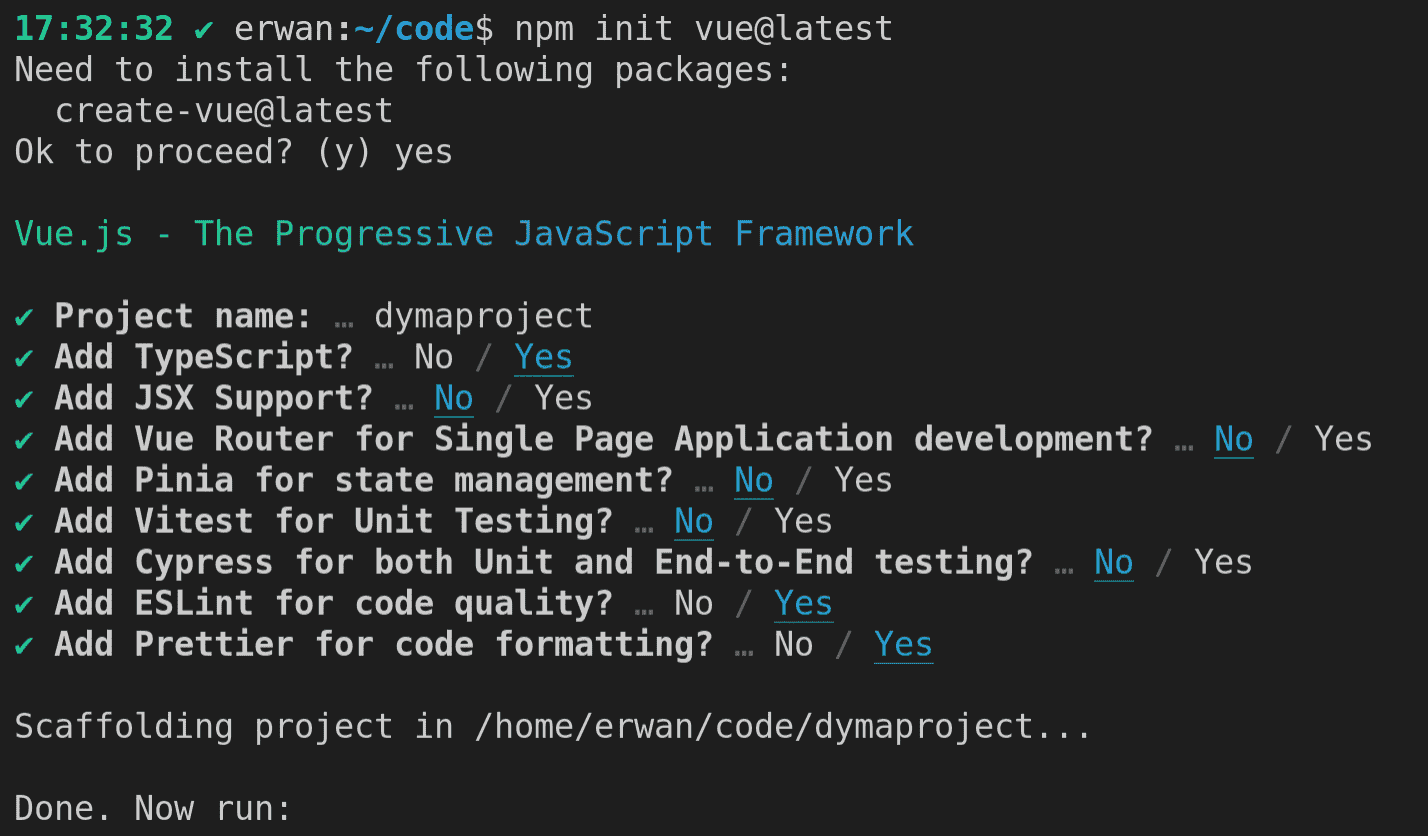
\includegraphics[width=10cm]{images/image04.png}
\end{center}

Allez dans le dossier :
\begin{minted}[
mathescape,
framesep=2mm,
baselinestretch=1.2,
%fontsize=\footnotesize,
bgcolor=LightGray,
%linenos
]{bash}
cd boutique
\end{minted}
Bien sûr adaptez {\color{monOrange}boutique} avec le nom que vous avez donné au projet.

Installez les dépendances :
\begin{minted}[
mathescape,
framesep=2mm,
baselinestretch=1.2,
%fontsize=\footnotesize,
bgcolor=LightGray,
%linenos
]{bash}
npm install
\end{minted}
Ouvrez {\color{monOrange}VS Code} et chargez le projet :
\begin{minted}[
mathescape,
framesep=2mm,
baselinestretch=1.2,
%fontsize=\footnotesize,
bgcolor=LightGray,
%linenos
]{bash}
code .
\end{minted}

\subsection{Inclusion d'une police}
Nous modifions {\color{monOrange}index.html} pour charger une police depuis {\color{monOrange}Google API} :
\begin{minted}[
mathescape,
framesep=2mm,
baselinestretch=1.2,
%fontsize=\footnotesize,
bgcolor=LightGray,
%linenos
]{html}
<!DOCTYPE html>
<html lang="fr">
  <head>
    <meta charset="UTF-8" />
    <link rel="icon" href="/favicon.ico" />
    <meta name="viewport" content="width=device-width, initial-scale=1.0" />
    <title>Vite App</title>
    <link rel="preconnect" href="https://fonts.googleapis.com" />
    <link rel="preconnect" href="https://fonts.gstatic.com" crossorigin />
    <link
      href="https://fonts.googleapis.com/css2?family=Roboto:wght@400;500;700&display=swap"
      rel="stylesheet"
    />
  </head>
  <body>
    <div id="app"></div>
    <script type="module" src="/src/main.ts"></script>
  </body>
</html>
\end{minted}

\subsection{Modification de {\color{monOrange}App.vue}}
Nous enlevons tout le code par défaut et ajoutons l'utilisation de {\color{monOrange}scss} :
\begin{minted}[
mathescape,
framesep=2mm,
baselinestretch=1.2,
%fontsize=\footnotesize,
bgcolor=LightGray,
%linenos
]{html}
<script setup lang="ts"></script>

<template>
  <h1>Bonjour le monde !</h1>
</template>

<style lang="scss">
@use './assets/base.scss' as *;
</style>
\end{minted}

\subsection{Installation de {\color{monOrange}Sass}}
Installez Sass en dépendance de développement :
\begin{minted}[
mathescape,
framesep=2mm,
baselinestretch=1.2,
%fontsize=\footnotesize,
bgcolor=LightGray,
%linenos
]{bash}
npm i -D sass
\end{minted}

\subsection{Modification de {\color{monOrange}assets/base.css}}
Renommez le fichier {\color{monOrange}base.css} en {\color{monOrange}base.scss} car nous utilisons {\color{monOrange}Sass} et mettez pour le moment :
\begin{minted}[
mathescape,
framesep=2mm,
baselinestretch=1.2,
%fontsize=\footnotesize,
bgcolor=LightGray,
%linenos
]{scss}
:root {
  --font-family: 'Roboto', sans-serif;
}

body {
  font-family: var(--font-family);
}
\end{minted}

\subsection{Installation de l'extension pour navigateur {\color{monOrange}Vue}}
Installez l'extension Chrome pour Vue.js ou l'extension Firefox suivant votre navigateur.

Le nom de l'extension est Vue.js devtools.

\subsection{Extensions pour {\color{monOrange}Visual Studio Code}}
Vérifiez dans extensions sur VS Code que vous avez bien installé Volar et Volar TypeScript.

Vérifiez que l'extension {\color{monOrange}@builtin typescript} est bien désactivée pour le {\color{monOrange}workspace}.

%Exemple exécutable de la vidéo
%Vous pouvez directement utiliser ce code exécutable. N'hésitez pas à l'ouvrir dans un nouvel onglet pour le modifier ou mieux voir :

%%%%%%%%%%%%%%%%%%%%%%%%%%%%%%%%%%%%%%%%%%%%%%%%%%%%%%%%%%

\section{Mise en place du style}
\subsection{Modification deassets/base.scss}
Utilisez le style de base suivant :
\begin{minted}[
mathescape,
framesep=2mm,
baselinestretch=1.2,
fontsize=\footnotesize,
bgcolor=LightGray,
%linenos
]{scss}
:root {
  --primary-1: #3498db;
  --primary-2: #2980b9;
  --danger-1: #e74c3c;
  --danger-2: #c0392b;
  --success-1: #2ecc71;
  --success-2: #27ae60;
  --gray-1: #f6f6f6;
  --gray-2: #ddd;
  --gray-3: #34495e;
  --text-color: #444;
  --text-primary-color: #ffffff;

  --border: 1px solid var(--gray-2);
  --border-radius: 4px;

  --font-family: 'Roboto', sans-serif;
}
// reset
* {
  box-sizing: border-box;
}
h1,h2,h3,h4 {
  margin: 0;
}
ul {
  list-style: none;
  padding: 0;
}
img {
  max-width: 100%;
}
a {
  color: var(--text-color);
  text-decoration: none;
}
body {
  min-height: 100vh;
  padding: 0;
  margin: 0;
  font-family: var(--font-family);
  color: var(--text-color);
  background-color: var(--gray-1);
}
// flex
.d-flex {  display: flex; }
.flex-row {  flex-direction: row; }
.flex-column { flex-direction: column; }
.justify-content-center {  justify-content: center; }
.align-items-center {  align-items: center; }
.flex-fill {  flex: 1 1 auto; }
// padding
.p-10 {  padding: 10px; }
.p-20 {  padding: 20px; }
.p-30 {  padding: 30px; }
// margin
.m-10 {  margin: 10px; }
.m-20 {  margin: 20px; }
.m-30 {  margin: 30px; }
\end{minted}

Si vous ne maîtrisez pas certaines propriétés, n'hésitez pas à revoir les chapitres correspondants dans la formation HTML \& CSS.

\subsection{Création du fichier assets/debug.scss}
Créez les classes pour le débug plus facile du CSS :
\begin{minted}[
mathescape,
framesep=2mm,
baselinestretch=1.2,
fontsize=\footnotesize,
bgcolor=LightGray,
%linenos
]{css}
.b1 {  background-color: red; }
.b2 {  background-color: blue; }
.b3 {  background-color: yellow; }
.b4 {  background-color: green; }
.b5 {  background-color: purple; }
\end{minted}

Photocopieuse
\subsection{Modification de App.vue}
N'oubliez pas de modifier App.vue pour l'importer :
\begin{minted}[
mathescape,
framesep=2mm,
baselinestretch=1.2,
%fontsize=\footnotesize,
bgcolor=LightGray,
%linenos
]{html}
<script setup lang="ts"></script>

<template>
  <h1>Bonjour le monde !</h1>
</template>

<style lang="scss">
@use './assets/base.scss' as *;
@use './assets/debug.scss' as *;
</style>
\end{minted}

%Exemple exécutable de la vidéo
%Vous pouvez directement utiliser ce code exécutable. N'hésitez pas à l'ouvrir dans un nouvel onglet pour le modifier ou mieux voir :

%%%%%%%%%%%%%%%%%%%%%%%%%%%%%%%%%%%%%%%%%%%%%%%%%%%%%%%%%%%%%%

\section{Mise en page globale}
\subsection{Création de l'architecture}
Créez un dossier {\color{monOrange}components} dans le dossier {\color{monOrange}src}.

Dans ce dossier, créez les fichiers {\color{monOrange}Footer.vue, Header.vue, Shop.vue} et {\color{monOrange}Cart.vue}.

\subsubsection{Composant {\color{monOrange}Footer.vue}}
Mettez dans le composant :
\begin{minted}[
mathescape,
framesep=2mm,
baselinestretch=1.2,
fontsize=\footnotesize,
bgcolor=LightGray,
%linenos
]{html}
<script setup lang="ts"></script>

<template>
  <footer>
    <h1>Footer</h1>
  </footer>
</template>

<style lang="scss" scoped></style>
\end{minted}

\subsubsection{Composant {\color{monOrange}Header.vue}}
Mettez dans le composant :
\begin{minted}[
mathescape,
framesep=2mm,
baselinestretch=1.2,
fontsize=\footnotesize,
bgcolor=LightGray,
%linenos
]{html}
<script setup lang="ts"></script>

<template>
  <header>
    <h1>Header</h1>
  </header>
</template>

<style lang="scss" scoped></style>
\end{minted}

\subsubsection{Composant {\color{monOrange}Shop.vue}}
Mettez dans le composant :
\begin{minted}[
mathescape,
framesep=2mm,
baselinestretch=1.2,
fontsize=\footnotesize,
bgcolor=LightGray,
%linenos
]{html}
<script setup lang="ts"></script>

<template>
  <div>
    <h1>Shop</h1>
  </div>
</template>

<style lang="scss" scoped></style>
\end{minted}

\subsubsection{Composant {\color{monOrange}Cart.vue}}
Mettez dans le composant :
\begin{minted}[
mathescape,
framesep=2mm,
baselinestretch=1.2,
fontsize=\footnotesize,
bgcolor=LightGray,
%linenos
]{html}
<script setup lang="ts"></script>

<template>
  <div>
    <h1>Cart</h1>
  </div>
</template>

<style lang="scss" scoped></style>
\end{minted}

Notez que nous utilisons {\color{monOrange}scoped} pour limiter la portée des styles déclarés dans ces composants.

\subsubsection{Modification de {\color{monOrange}App.vue}}
Modifications de notre composant racine pour importer et utiliser les composants que nous avons créés :
\begin{minted}[
mathescape,
framesep=2mm,
baselinestretch=1.2,
fontsize=\footnotesize,
bgcolor=LightGray,
%linenos
]{html}
<script setup lang="ts">
import TheHeader from './components/Header.vue';
import TheFooter from './components/Footer.vue';
import Shop from './components/Shop.vue';
import Cart from './components/Cart.vue';
</script>

<template>
  <div class="app-container">
    <TheHeader class="header b1" />
    <Shop class="shop b2" />
    <Cart class="cart b3" />
    <TheFooter class="footer b4" />
  </div>
</template>

<style lang="scss">
@use './assets/base.scss' as *;
@use './assets/debug.scss' as *;

.app-container {
  min-height: 100vh;
  display: grid;
  grid-template-areas: 'header header' 'shop cart' 'footer footer';
  grid-template-columns: 75% 25%;
  grid-template-rows: 48px auto 48px;
}
.header {  grid-area: header; }
.shop {  grid-area: shop; }
.cart {  grid-area: cart; }
.footer {  grid-area: footer; }
</style>
\end{minted}

{\em Nous utilisons une grille {\color{monOrange}CSS}, n'hésitez pas à revoir le chapitre sur les grilles dans la formation {\color{monOrange}CSS}}.

%Exemple exécutable de la vidéo
%Vous pouvez directement utiliser ce code exécutable. N'hésitez pas à l'ouvrir dans un nouvel onglet pour le modifier ou mieux voir :

%%%%%%%%%%%%%%%%%%%%%%%%%%%%%%%%%%%%%%%%%%%%%%%%%%%%%%%%%%%%

\section{Mise en page boutique et panier}
\subsection{Architecture}
Dans le dossier components créez un dossier Cart et un dossier Shop.

Déplacez le composant Cart.vue dans Cart et Shop.vue dans Shop.

Commencez à jour les chemins d'imports dans App.vue :
\begin{minted}[
mathescape,
framesep=2mm,
baselinestretch=1.2,
fontsize=\footnotesize,
bgcolor=LightGray,
%linenos
]{html}
<script setup lang="ts">
import TheHeader from './components/Header.vue';
import TheFooter from './components/Footer.vue';
import Shop from './components/Shop/Shop.vue';
import Cart from './components/Cart/Cart.vue';
</script>
\end{minted}

Dans le dossier Cart, créez les composants CartProductList.vue et CartProduct.vue.

Même choisi dans le dossier Shop, créé deux composants ShopProductList.vue et ShopProduct.vue.

\subsection{Modification de {\color{monOrange}Shop.vue}}
Nous allons importer et utiliser les nouveaux composants relatifs à la liste des produits :
\begin{minted}[
mathescape,
framesep=2mm,
baselinestretch=1.2,
fontsize=\footnotesize,
bgcolor=LightGray,
%linenos
]{html}
<script setup lang="ts">
import ShopProductList from './ShopProductList.vue';
</script>

<template>
  <div>
    <ShopProductList />
  </div>
</template>

<style lang="scss" scoped></style>
\end{minted}
Dans ce composant nous plaçons le composant qui va être responsable de gérer la liste des produits.

\subsection{Modification de ShopProductList.vue}
Dans ce composant nous allons utiliser plusieurs instances de notre composant ShopProduct et les disposer en utilisant une grille CSS :
\begin{minted}[
mathescape,
framesep=2mm,
baselinestretch=1.2,
fontsize=\footnotesize,
bgcolor=LightGray,
%linenos
]{html}
<script setup lang="ts">
import ShopProduct from './ShopProduct.vue';
</script>

<template>
  <div class="grid p-20">
    <ShopProduct />
    <ShopProduct />
    <ShopProduct />
    <ShopProduct />
    <ShopProduct />
    <ShopProduct />
    <ShopProduct />
    <ShopProduct />
    <ShopProduct />
  </div>
</template>

<style lang="scss" scoped>
.grid {
  display: grid;
  grid-template-columns: 1fr 1fr 1fr 1fr;
  grid-auto-rows: 300px;
  gap: 20px;
}
</style>
\end{minted}

\subsection{Modification de ShopProduct.vue}
Dans ce composant nous affichons juste un titre pour le moment :
\begin{minted}[
mathescape,
framesep=2mm,
baselinestretch=1.2,
fontsize=\footnotesize,
bgcolor=LightGray,
%linenos
]{html}
<script setup lang="ts"></script>

<template>
  <div class="b5">
    <h1>Shop Product</h1>
  </div>
</template>

<style lang="scss" scoped></style>
\end{minted}

\subsection{Modification de Cart.vue}
Dans ce composant nous utilisons le composant CartProductList responsable de gérer l'affichage des produits du panier :
\begin{minted}[
mathescape,
framesep=2mm,
baselinestretch=1.2,
fontsize=\footnotesize,
bgcolor=LightGray,
%linenos
]{html}
<script setup lang="ts">
import CartProductList from './CartProductList.vue';
</script>

<template>
  <div class="p-20">
    <h2 class="mb-10">Panier</h2>
    <CartProductList />
  </div>
</template>

<style lang="scss" scoped></style>
\end{minted}

N'oubliez pas de modifier assets/base.scss pour ajouter la classe mb-10 :
\begin{minted}[
mathescape,
framesep=2mm,
baselinestretch=1.2,
fontsize=\footnotesize,
bgcolor=LightGray,
%linenos
]{html}
.mb-10 {
  margin-bottom: 10px;
}
\end{minted}

\subsection{Modification de CartProductList.vue}
Dans ce composant nous allons utiliser plusieurs instances du composant CartProduct qui sont les produits dans le panier.

Nous utilisons des boîtes flexibles pour positionner les produits.
\begin{minted}[
mathescape,
framesep=2mm,
baselinestretch=1.2,
fontsize=\footnotesize,
bgcolor=LightGray,
%linenos
]{html}
<script setup lang="ts">
import CartProduct from './CartProduct.vue';
</script>

<template>
  <div class="d-flex flex-column">
    <CartProduct />
    <CartProduct />
    <CartProduct />
    <CartProduct />
    <CartProduct />
    <CartProduct />
  </div>
</template>

<style lang="scss" scoped></style>
\end{minted}

\subsection{Modification de CartProduct.vue}
Dans ce composant nous affichons pour le moment simplement un titre :
\begin{minted}[
mathescape,
framesep=2mm,
baselinestretch=1.2,
fontsize=\footnotesize,
bgcolor=LightGray,
%linenos
]{html}
<script setup lang="ts"></script>

<template>
  <div class="mb-10 b5">
    <h1>Product</h1>
  </div>
</template>

<style lang="scss" scoped></style>
\end{minted}

%Exemple exécutable de la vidéo
%Vous pouvez directement utiliser ce code exécutable. N'hésitez pas à l'ouvrir dans un nouvel onglet pour le modifier ou mieux voir :

%%%%%%%%%%%%%%%%%%%%%%%%%%%%%%%%%%%%%%%%%%%%%%%%%%%%%%%%%%%%%%

\section{Mise en page du header et du footer}
\subsection{Modification deassets/base.scss}
Ajoutez les classes utilitaires dont nous aurons besoin :
\begin{minted}[
mathescape,
framesep=2mm,
baselinestretch=1.2,
fontsize=\footnotesize,
bgcolor=LightGray,
%linenos
]{css}
.px-20 {
  padding-left: 20px;
  padding-right: 20px;
}
.p-30 { padding: 30px; }
// margin
.m-10 { margin: 10px; }
.mb-10 { margin-bottom: 10px; }
.mr-10 { margin-right: 10px; }
.mr-20 {  margin-right: 20px; }
\end{minted}

\subsection{Modification de Header.vue}
Nous mettons en place notre header :
\begin{minted}[
mathescape,
framesep=2mm,
baselinestretch=1.2,
fontsize=\footnotesize,
bgcolor=LightGray,
%linenos
]{html}
<script setup lang="ts"></script>

<template>
  <header class="px-20 d-flex flex-row align-items-center">
    <a href="#" class="d-flex flex-row align-items-center mr-20">
      <img src="../assets/logo.svg" />
      <span class="logo">Dyma</span>
    </a>
    <ul class="d-flex flex-row flex-fill">
      <li class="mr-10">
        <a href="#">Boutique</a>
      </li>
      <li>
        <a href="#">Admin</a>
      </li>
    </ul>
    <ul class="d-flex flex-row">
      <li class="mr-10">
        <a href="#">Inscription</a>
      </li>
      <li>
        <a href="#">Connexion</a>
      </li>
    </ul>
  </header>
</template>

<style lang="scss" scoped>
header {
  background-color: var(--primary-1);
  a {
    color: var(--text-primary-color);
    img {
      width: 20px;
      margin-right: 5px;
    }
    .logo {
      font-weight: 700;
      font-size: 20px;
    }
  }
}
</style>
\end{minted}

\subsection{Modification de Footer.vue}
Nous mettons en place notre footer :
\begin{minted}[
mathescape,
framesep=2mm,
baselinestretch=1.2,
fontsize=\footnotesize,
bgcolor=LightGray,
%linenos
]{html}
<script setup lang="ts"></script>

<template>
  <footer class="d-flex flex-row justify-content-center align-items-center">
    <p>Copyright © 2014-2022 Dyma</p>
  </footer>
</template>

<style lang="scss" scoped>
footer {
  background-color: var(--gray-3);
  color: var(--text-primary-color);
}
</style>
\end{minted}

%Exemple exécutable de la vidéo
%Vous pouvez directement utiliser ce code exécutable. N'hésitez pas à l'ouvrir dans un nouvel onglet pour le modifier ou mieux voir :

%%%%%%%%%%%%%%%%%%%%%%%%%%%%%%%%%%%%%%%%%%%%%%%%%%%%%%%%%%%

\section{Mise en page de la partie Shop}
\subsection{Modification de {\color{monOrange}ShopProduct.vue}}
Nous mettons pour le moment les détails du produit en dur :
\begin{minted}[
mathescape,
framesep=2mm,
baselinestretch=1.2,
fontsize=\footnotesize,
bgcolor=LightGray,
%linenos
]{html}
<script setup lang="ts"></script>

<template>
  <div class="product d-flex flex-column">
    <div class="product-image"></div>
    <div class="p-10 d-flex flex-column">
      <h4>Macbook Pro</h4>
      <p>Performances exceptionnelles avec la puce M1 Pro ou M1</p>
      <div class="d-flex flex-row align-items-center">
        <strong class="flex-fill">Prix : 1500€</strong>
        <button class="btn btn-primary">Ajouter au panier</button>
      </div>
    </div>
  </div>
</template>

<style lang="scss" scoped>
.product {
  background-color: #ffffff;
  border: var(--border);
  border-radius: var(--border-radius);
  &-image {
    border-top-right-radius: var(--border-radius);
    border-top-left-radius: var(--border-radius);
    background-image: url('https://media.ldlc.com/r1600/ld/products/00/05/82/01/LD0005820198_1.jpg');
    background-size: cover;
    background-position: center;
    height: 250px;
  }
}
</style>
\end{minted}

Photocopieuse
\subsection{Classes pour les boutons}
Modifiez {\color{monOrange}assets/base.scss} pour ajouter les classes pour nos boutons :
\begin{minted}[
mathescape,
framesep=2mm,
baselinestretch=1.2,
fontsize=\footnotesize,
bgcolor=LightGray,
%linenos
]{scss}
// buttons

.btn {
  padding: 8px 15px;
  border: 0;
  border-radius: var(--border-radius);
  cursor: pointer;
  font-weight: 500;
  transition: background-color 0.2s;
}

.btn-primary {
  background-color: var(--primary-1);
  color: var(--text-primary-color);
  &:hover {
    background-color: var(--primary-2);
  }
}

.btn-danger {
  background-color: var(--danger-1);
  color: var(--text-primary-color);
  &:hover {
    background-color: var(--danger-2);
  }
}
\end{minted}

%Exemple exécutable de la vidéo
%Vous pouvez directement utiliser ce code exécutable. N'hésitez pas à l'ouvrir dans un nouvel onglet pour le modifier ou mieux voir :

%%%%%%%%%%%%%%%%%%%%%%%%%%%%%%%%%%%%%%%%%%%%%%%%%%%%%%%%%%%%%%%%

\section{Mise en place du panier}
\subsection{Modification de {\color{monOrange}CartProduct.vue}}
Nous mettons en place en dur le produit du panier pour terminer la mise en page :
\begin{minted}[
mathescape,
framesep=2mm,
baselinestretch=1.2,
fontsize=\footnotesize,
bgcolor=LightGray,
%linenos
]{html}
<script setup lang="ts"></script>

<template>
  <div class="mb-10 p-10 d-flex flex-row align-items-center product">
    <strong class="flex-fill mr-10">Macbook Pro</strong>
    <span class="mr-10">Prix : 1500€</span>
    <button class="btn btn-danger">Supprimer</button>
  </div>
</template>

<style lang="scss" scoped>
.product {
  border: var(--border);
  border-radius: var(--border-radius);
  background-color: var(--gray-1);
}
</style>
\end{minted}

\subsection{Modification de {\color{monOrange}App.vue}}
Nous modifions légèrement la classe {\color{monOrange}cart} :
\begin{minted}[
mathescape,
framesep=2mm,
baselinestretch=1.2,
fontsize=\footnotesize,
bgcolor=LightGray,
%linenos
]{html}
<style lang="scss">
@use './assets/base.scss' as *;
@use './assets/debug.scss' as *;

.app-container {
  min-height: 100vh;
  display: grid;
  grid-template-areas: 'header header' 'shop cart' 'footer footer';
  grid-template-columns: 75% 25%;
  grid-template-rows: 48px auto 48px;
}
.header {
  grid-area: header;
}
.shop {
  grid-area: shop;
}
.cart {
  grid-area: cart;
  border-left: var(--border);
  background-color: white;
}
.footer {
  grid-area: footer;
}
</style> 
\end{minted}
%Exemple exécutable de la vidéo
%Vous pouvez directement utiliser ce code exécutable. N'hésitez pas à l'ouvrir dans un nouvel onglet pour le modifier ou mieux voir :
%%%%%%%%%%%%%%%%%%%%%%%%%%%%%%%%%%%%%%%%%%%%%%%%%%%%%%
\section{Utilisation des props pour les produits}
\subsection{Création des interfaces}
Créez un dossier interfaces dans src.

Créer dans ce dossier un fichier Product.interface.ts :
\begin{minted}[
mathescape,
framesep=2mm,
baselinestretch=1.2,
fontsize=\footnotesize,
bgcolor=LightGray,
%linenos
]{javascript}
export interface ProductInterface {
    title: string;
    image: string;
    price: number;
    description: string;
}
\end{minted}
\subsection{Données en dur}
En attendant d'avancer plus dans le projet et d'utiliser des requêtes HTTP pour récupérer les produits, nous allons mettre les données en dur.

Pour ce faire, créez un dossier data dans src.

Dans ce dossier, créez un fichier product.ts :
\begin{minted}[
mathescape,
framesep=2mm,
baselinestretch=1.2,
fontsize=\footnotesize,
bgcolor=LightGray,
%linenos
]{javascript}
export default [
  {
    id: 1,
    image: 'src/assets/images/macbookpro.PNG',
    title: 'Macbook Pro',
    description:
      'Lorem ipsum dolor sit amet consectetur adipisicing edolor tempore ipsam cum ipsum reiciendis',
    price: 1500,
  },
  {
    id: 2,
    image: 'src/assets/images/levono.PNG',
    title: 'Levono Pro',
    description:
      'Lorem ipsum dolor sit amet consectetur adipisicing edolor tempore ipsam cum ipsum reiciendis',
    price: 2300,
  },
  {
    id: 3,
    image: 'src/assets/images/rider.PNG',
    title: 'Rider',
    description:
      'Lorem ipsum dolor sit amet consectetur adipisicing edolor tempore ipsam cum ipsum reiciendis',
    price: 1200,
  },
  {
    id: 4,
    image: 'src/assets/images/ldlc.PNG',
    title: 'LDLC benolo',
    description:
      'Lorem ipsum dolor sit amet consectetur adipisicing edolor tempore ipsam cum ipsum reiciendis',
    price: 4500,
  },
  {
    id: 5,
    image: 'src/assets/images/asus.PNG',
    title: 'Asus gamer',
    description:
      'Lorem ipsum dolor sit amet consectetur adipisicing edolor tempore ipsam cum ipsum reiciendis',
    price: 3755,
  },
  {
    id: 6,
    image: 'src/assets/images/rog.PNG',
    title: 'Rog desktop',
    description:
      'Lorem ipsum dolor sit amet consectetur adipisicing edolor tempore ipsam cum ipsum reiciendis',
    price: 2452,
  },
  {
    id: 7,
    image: 'src/assets/images/msi.PNG',
    title: 'MSI play',
    description:
      'Lorem ipsum dolor sit amet consectetur adipisicing edolor tempore ipsam cum ipsum reiciendis',
    price: 1478,
  },
  {
    id: 8,
    image: 'src/assets/images/pad.PNG',
    title: 'Think pad',
    description:
      'Lorem ipsum dolor sit amet consectetur adipisicing edolor tempore ipsam cum ipsum reiciendis',
    price: 899,
  },
];
\end{minted}
\subsection{Modification de App.vue}
Dans le composant racine, nous allons importer les données et les typer dans une propriété réactive.

Nous allons ensuite les passer à notre composant enfant Shop en utilisant une liaison de données avec v-bind.
\begin{minted}[
mathescape,
framesep=2mm,
baselinestretch=1.2,
fontsize=\footnotesize,
bgcolor=LightGray,
%linenos
]{html}
<script setup lang="ts">
import TheHeader from './components/Header.vue';
import TheFooter from './components/Footer.vue';
import Shop from './components/Shop/Shop.vue';
import Cart from './components/Cart/Cart.vue';
import data from './data/product';

import { reactive } from 'vue';
import type { ProductInterface } from './interfaces';
const products = reactive<ProductInterface[]>(data);
</script>

<template>
  <div class="app-container">
    <TheHeader class="header" />
    <Shop :products="products" class="shop" />
    <Cart class="cart" />
    <TheFooter class="footer" />
  </div>
</template>

<style lang="scss">
@use './assets/base.scss' as *;
@use './assets/debug.scss' as *;

.app-container {
  min-height: 100vh;
  display: grid;
  grid-template-areas: 'header header' 'shop cart' 'footer footer';
  grid-template-columns: 75% 25%;
  grid-template-rows: 48px auto 48px;
}
.header {
  grid-area: header;
}
.shop {
  grid-area: shop;
}
.cart {
  grid-area: cart;
  border-left: var(--border);
  background-color: white;
}
.footer {
  grid-area: footer;
}
</style>
\end{minted}
{\tt reactive<ProductInterface[]>(data)} : nous passons en type générique un tableau de produits qui doivent respecter l'interface {\color{monOrange}ProductInterface}. Nous initialisons la propriété réactive avec nos données contenues dans {\color{monOrange}data}.

\subsection{Modification de {\color{monOrange}Shop.vue}}
Dans le composant {\color{monOrange}Shop.vue}, nous définissons la {\color{monOrange}prop} reçue depuis le composant parent grâce à {\color{monOrange}defineProps}, à savoir la liste de tous les produits.

Nous typons la {\color{monOrange}props} en passant le type générique {\tt  \{ products: ProductInterface[] \}} : cela signifie que nous recevons un objet contenant une propriété {\color{monOrange}products} qui a pour valeur un tableau contenant des {\color{monOrange}ProductInterface}.

Nous repassons ensuite la {\color{monOrange}prop} reçue plus bas dans l'arbre :
\begin{minted}[
mathescape,
framesep=2mm,
baselinestretch=1.2,
fontsize=\footnotesize,
bgcolor=LightGray,
%linenos
]{html}
<script setup lang="ts">
import type { ProductInterface } from '@/interfaces';
import ShopProductList from './ShopProductList.vue';

defineProps<{
  products: ProductInterface[];
}>();
</script>

<template>
  <div>
    <ShopProductList :products="products" />
  </div>
</template>

<style lang="scss" scoped></style>
\end{minted}
\subsection{Modification de {\color{monOrange}ShopProductList.vue}}
Dans le composant {\color{monOrange}ShopProductList}, nous récupérons également la {\color{monOrange}prop} que nous typons comme dans le composant parent {\color{monOrange}Shop}.

Cette fois, nous utilisons la directive {\color{monOrange}v-for} pour boucler sur les produits et nous utilisons une liaison de propriété pour passer le produit à chaque instance du composant {\color{monOrange}ShopProduct}.
\begin{minted}[
mathescape,
framesep=2mm,
baselinestretch=1.2,
fontsize=\footnotesize,
bgcolor=LightGray,
%linenos
]{html}
<script setup lang="ts">
import type { ProductInterface } from '@/interfaces';
import ShopProduct from './ShopProduct.vue';
defineProps<{
  products: ProductInterface[];
}>();
</script>

<template>
  <div class="grid p-20">
    <ShopProduct v-for="product of products" :product="product" />
  </div>
</template>

<style lang="scss" scoped>
.grid {
  display: grid;
  grid-template-columns: 1fr 1fr 1fr 1fr;
  grid-auto-rows: 400px;
  gap: 20px;
}
</style>
\end{minted}
\subsection{Modification de {\color{monOrange}ShopProduct.vue}}
Dans le composant {\color{monOrange}ShopProduct}, nous récupérons le produit en {\color{monOrange}props} et nous utilisons la notation raccourcie de la directive {\color{monOrange}v-text} pour afficher les différentes propriétés du produit.
\begin{minted}[
mathescape,
framesep=2mm,
baselinestretch=1.2,
fontsize=\footnotesize,
bgcolor=LightGray,
%linenos
]{scss}
<script setup lang="ts">
import type { ProductInterface } from '@/interfaces';
defineProps<{
  product: ProductInterface;
}>();
</script>

<template>
  <div class="product d-flex flex-column">
    <div
      class="product-image"
      :style="{ backgroundImage: `url(${product.image})` }"
    ></div>
    <div class="p-10 d-flex flex-column">
      <h4>{{ product.title }}</h4>
      <p>{{ product.description }}</p>
      <div class="d-flex flex-row align-items-center">
        <strong class="flex-fill">Prix : {{ product.price }}€</strong>
        <button class="btn btn-primary">Ajouter au panier</button>
      </div>
    </div>
  </div>
</template>

<style lang="scss" scoped>
.product {
  background-color: #ffffff;
  border: var(--border);
  border-radius: var(--border-radius);
  &-image {
    border-top-right-radius: var(--border-radius);
    border-top-left-radius: var(--border-radius);
    background-size: cover;
    background-position: center;
    height: 250px;
  }
}
</style>
\end{minted} 

%Exemple exécutable de la vidéo
%Vous pouvez directement utiliser ce code exécutable. N'hésitez pas à l'ouvrir dans un nouvel onglet pour le modifier ou mieux voir :

%%%%%%%%%%%%%%%%%%%%%%%%%%%%%%%%%%%%%%%%%%%%%%%%%%%%%%%%%%%%%%%

\section{Ajout d'un produit dans le panier}
\subsection{Logique à mettre en place}
De la même manière que nous faisons descendre la liste de produits dans l'arbre des composants dans cet ordre {\tt App $\to$ Shop $\to$ ShopProductList $\to$ ShopProduct}, nous souhaitons maintenant propager de l'information dans ce sens :
\begin{center}
{\tt  ShopProduct $\to$ ShopProductList $\to$ Shop $\to$ App}.
\end{center}

En effet, nous souhaitons que lorsqu'un utilisateur clique sur le bouton d'ajout au panier dans un composant {\color{monOrange}ShopProduct}, que cet événement remonte le long de l'arbre des composants et qu'il puisse nous informer sur quel produit l'utilisateur souhaite ajouter.

Pour ce faire, nous allons utiliser un événement personnalisé, qui contiendra l'{\color{monOrange}id} du produit à ajouter au panier. Cet événement sera émis depuis le composant {\color{monOrange}ShopProduct} concerné, puis sera réémis par {\color{monOrange}ShopProductList} puis par {\color{monOrange}Shop}.

Une fois que l'événement est arrivé au composant {\color{monOrange}App}, nous pourrons utiliser l'{\color{monOrange}id} du produit pour l'ajouter au panier. En effet, dans notre composant {\color{monOrange}App} nous centralisons les informations relatives au panier et aux produits.

\subsection{Modification de {\color{monOrange}App.vue}}
Dans le composant racine, nous modifions notre propriété réactive pour ajouter une propriété {\color{monOrange}cart} contenant les produits du panier. Nous initialisons le panier avec un tableau vide.

Nous créons une fonction {\color{monOrange}addProductToCart()} qui va permettre d'ajouter un produit dans le panier en utilisant son id unique. La logique est simple : nous récupérons le produit à l'aide de son id depuis la propriété réactive {\color{monOrange}state}, ensuite nous vérifions qu'il n'est pas déjà dans le panier, et enfin nous l'ajoutons au panier.

Notez bien que nous utilisons {\color{monOrange}\{ ...product \}} pour créer une copie de l'objet qui ne soit pas un {\color{monOrange}Proxy} vers l'objet du produit contenu dans la propriété réactive.

rappelez-vous en effet que les propriétés réactives contiennent des {\color{monOrange}Proxys} vers les objets que nous passons.

De cette manière, nous obtenons un nouvel objet qui a une nouvelle référence et qui est totalement différent de l'objet dans la propriété réactive.

Nous créons également un événement personnalisé {\color{monOrange}@add-product-to-cart} qui va déclencher la fonction {\color{monOrange}addProductToCart()} lorsqu'il est reçu. Ici, {\color{monOrange}addProductToCart()} est donc le gestionnaire pour cet événement.

Notez bien que l'événement personnalisé est en {\color{monOrange}kebab-case}.
\begin{minted}[
mathescape,
framesep=2mm,
baselinestretch=1.2,
fontsize=\footnotesize,
bgcolor=LightGray,
%linenos
]{html}
<script setup lang="ts">
import TheHeader from './components/Header.vue';
import TheFooter from './components/Footer.vue';
import Shop from './components/Shop/Shop.vue';
import Cart from './components/Cart/Cart.vue';
import data from './data/product';

import { reactive } from 'vue';
import type { ProductInterface } from './interfaces';

const state = reactive<{
  products: ProductInterface[];
  cart: ProductInterface[];
}>({
  products: data,
  cart: [],
});

function addProductToCart(productId: number): void {
  const product = state.products.find((product) => product.id === productId);
  if (product && !state.cart.find((product) => product.id === productId)) {
    state.cart.push({ ...product });
  }
}
</script>

<template>
  <div class="app-container">
    <TheHeader class="header" />
    <Shop
      :products="state.products"
      @add-product-to-cart="addProductToCart"
      class="shop"
    />
    <Cart class="cart" />
    <TheFooter class="footer" />
  </div>
</template>

<style lang="scss">
@use './assets/base.scss' as *;
@use './assets/debug.scss' as *;

.app-container {
  min-height: 100vh;
  display: grid;
  grid-template-areas: 'header header' 'shop cart' 'footer footer';
  grid-template-columns: 75% 25%;
  grid-template-rows: 48px auto 48px;
}
.header {
  grid-area: header;
}
.shop {
  grid-area: shop;
}
.cart {
  grid-area: cart;
  border-left: var(--border);
  background-color: white;
}
.footer {
  grid-area: footer;
}
</style>
\end{minted}
\subsection{Modification de {\color{monOrange}Shop.vue}}
Ici nous ajoutons la directive {\color{monOrange}v-on} pour écouter l'événement {\color{monOrange}add-product-to-cart} lorsqu'il est émis par le composant {\color{monOrange}ShopProductList}

Nous ne faisons que le retransmettre en démontrant un événement avec {\color{monOrange}defineEmits} qui est identique à celui reçu.

L'événement qui va être retransmis est {\color{monOrange}addProductToCart} (notez bien le {\color{monOrange}camelCase}) et il contient un seul argument qui est le {\color{monOrange}productId} de type {\color{monOrange}number}.
\begin{minted}[
mathescape,
framesep=2mm,
baselinestretch=1.2,
fontsize=\footnotesize,
bgcolor=LightGray,
%linenos
]{html}
<script setup lang="ts">
import type { ProductInterface } from '@/interfaces';
import ShopProductList from './ShopProductList.vue';

defineProps<{
  products: ProductInterface[];
}>();

const emit = defineEmits<{
  (e: 'addProductToCart', productId: number): void;
}>();
</script>

<template>
  <div>
    <ShopProductList
      @add-product-to-cart="emit('addProductToCart', $event)"
      :products="products"
    />
  </div>
</template>

<style lang="scss" scoped></style>
\end{minted}
%$
\subsection{Modification de {\color{monOrange}ShopProductList.vue}}
Même logique, nous ne faisons que retransmettre l'événement provenant du composant {\color{monOrange}ShopProduct} vers le composant {\color{monOrange}Shop} :
\begin{minted}[
mathescape,
framesep=2mm,
baselinestretch=1.2,
fontsize=\footnotesize,
bgcolor=LightGray,
%linenos
]{html}
<script setup lang="ts">
import type { ProductInterface } from '@/interfaces';
import ShopProduct from './ShopProduct.vue';

defineProps<{
  products: ProductInterface[];
}>();

const emit = defineEmits<{
  (e: 'addProductToCart', productId: number): void;
}>();
</script>

<template>
  <div class="grid p-20">
    <ShopProduct
      @add-product-to-cart="emit('addProductToCart', $event)"
      v-for="product of products"
      :product="product"
    />
  </div>
</template>

<style lang="scss" scoped>
.grid {
  display: grid;
  grid-template-columns: 1fr 1fr 1fr 1fr;
  grid-auto-rows: 400px;
  gap: 20px;
}
</style>
\end{minted}
%$
\subsection{Modification de {\color{monOrange}ShopProduct.vue}}
La logique est la suivante :

{\color{monOrange}@click} : Ici nous créons une liaison d'événement avec {\color{monOrange}v-on} sur l'événement {\color{monOrange}click} sur le bouton d'ajout au panier.

{\tt const emit = defineEmits<{ (e: 'addProductToCart', productId: number): void; }>();} : Nous créons un événement personnalisé {\tt 'addProductToCart'} qui va contenir un seul argument : le {\color{monOrange}productId}.

{\tt @click="emit('addProductToCart', product.id)"} : Nous l'émettons avec {\color{monOrange}emit()} lors d'un clic sur le bouton. Le premier argument est le nom de l'événement en {\color{monOrange}camelCase} et le deuxième argument est l'{\color{monOrange}id} du produit. Voici le code du composant :
\begin{minted}[
mathescape,
framesep=2mm,
baselinestretch=1.2,
fontsize=\footnotesize,
bgcolor=LightGray,
%linenos
]{html}
<script setup lang="ts">
import type { ProductInterface } from '@/interfaces';

defineProps<{
  product: ProductInterface;
}>();

const emit = defineEmits<{
  (e: 'addProductToCart', productId: number): void;
}>();
</script>

<template>
  <div class="product d-flex flex-column">
    <div
      class="product-image"
      :style="{ backgroundImage: `url(${product.image})` }"
    ></div>
    <div class="p-10 d-flex flex-column">
      <h4>{{ product.title }}</h4>
      <p>{{ product.description }}</p>
      <div class="d-flex flex-row align-items-center">
        <strong class="flex-fill">Prix : {{ product.price }}€</strong>
        <button
          class="btn btn-primary"
          @click="emit('addProductToCart', product.id)"
        >
          Ajouter au panier
        </button>
      </div>
    </div>
  </div>
</template>

<style lang="scss" scoped>
.product {
  background-color: #ffffff;
  border: var(--border);
  border-radius: var(--border-radius);
  &-image {
    border-top-right-radius: var(--border-radius);
    border-top-left-radius: var(--border-radius);
    background-size: cover;
    background-position: center;
    height: 250px;
  }
}
</style>
\end{minted}
%$
%Exemple exécutable de la vidéo
%Vous pouvez directement utiliser ce code exécutable. N'hésitez pas à l'ouvrir dans un nouvel onglet pour le modifier ou mieux voir :

%%%%%%%%%%%%%%%%%%%%%%%%%%%%%%%%%%%%%%%%%%%%%%%%%%%%%%%%

\section{Affichage et suppression pour la partie panier}
\subsection{Logique à mettre en place}
De la même manière que précédemment pour la partie {\color{monOrange}Shop}, nous souhaitons faire descendre l'information du contenu du panier le long de l'arbre des composants de cette manière :
\begin{center}
{\tt App $\to$ Cart $\to$ CartProductList $\to$ CartProduct}.
\end{center}
De cette manière, nous pourrons afficher le contenu du panier. Nous allons simplement utiliser une {\color{monOrange}prop} sur les différents niveaux de composants pour passer cette information.

Nous souhaitons également faire remonter l'information dans le sens inverse lorsque l'utilisateur clique sur le bouton "Supprimer" d'un élément du panier :

\begin{center}
{\tt CartProduct $\to$ CartProductList $\to$ Cart $\to$ App}.
\end{center}
Pour ce faire, nous allons utiliser un événement personnalisé, qui contiendra l'{\color{monOrange}id} du produit à supprimer du panier. Cet événement sera émis depuis le composant {\color{monOrange}CartProduct} concerné, puis sera réémis par {\color{monOrange}CartProductList} puis par {\color{monOrange}Cart}.

Une fois que l'événement sera arrivé au composant {\color{monOrange}App}, nous pourrons utiliser l'{\color{monOrange}id} du produit pour le supprimer du panier. La logique est donc similaire à celle utilisée pour la partie {\color{monOrange}Shop}.

\subsection{Modification de {\color{monOrange}App.vue}}
Dans {\color{monOrange}App.vue} :
\begin{minted}[
mathescape,
framesep=2mm,
baselinestretch=1.2,
fontsize=\footnotesize,
bgcolor=LightGray,
%linenos
]{html}
<script setup lang="ts">
import TheHeader from './components/Header.vue';
import TheFooter from './components/Footer.vue';
import Shop from './components/Shop/Shop.vue';
import Cart from './components/Cart/Cart.vue';
import data from './data/product';

import { reactive } from 'vue';
import type { ProductInterface } from './interfaces';

const state = reactive<{
  products: ProductInterface[];
  cart: ProductInterface[];
}>({
  products: data,
  cart: [],
});

function addProductToCart(productId: number): void {
  const product = state.products.find((product) => product.id === productId);
  if (product && !state.cart.find((product) => product.id === productId)) {
    state.cart.push({ ...product });
  }
}

function removeProductFromCart(productId: number): void {
  state.cart = state.cart.filter((product) => product.id !== productId);
}
</script>

<template>
  <div class="app-container">
    <TheHeader class="header" />
    <Shop
      :products="state.products"
      @add-product-to-cart="addProductToCart"
      class="shop"
    />
    <Cart
      :cart="state.cart"
      class="cart"
      @remove-product-from-cart="removeProductFromCart"
    />
    <TheFooter class="footer" />
  </div>
</template>

<style lang="scss">
@use './assets/base.scss' as *;
@use './assets/debug.scss' as *;

.app-container {
  min-height: 100vh;
  display: grid;
  grid-template-areas: 'header header' 'shop cart' 'footer footer';
  grid-template-columns: 75% 25%;
  grid-template-rows: 48px auto 48px;
}
.header {
  grid-area: header;
}
.shop {
  grid-area: shop;
}
.cart {
  grid-area: cart;
  border-left: var(--border);
  background-color: white;
}
.footer {
  grid-area: footer;
}
</style>
\end{minted}
Nous définissons une fonction {\color{monOrange}removeProductFromCart()} pour supprimer un article du panier lorsque nous recevons l'événement {\color{monOrange}removeProductFromCart}.
\begin{itemize}
\item {\tt @remove-product-from-cart="removeProductFromCart"} : nous écoutons l'événement {\color{monOrange}remove-product-from-cart} et enregistrons la fonction {\color{monOrange}removeProductFromCart()} comme gestionnaire d'événement.

Notez bien que nous n'utilisons pas de parenthèses avec {\color{monOrange}removeProductFromCart}. En JavaScript cela signifie que nous passons la fonction avec tous les arguments récupérés.

Notez également bien que l'événement côté {\color{monOrange}template} est en {\color{monOrange}kebab-case} ({\tt remove-product-from-cart}) et qu'il soit être en {\color{monOrange}camelCase} côté script ({\tt removeProductFromCart}).

\item {\tt :cart="state.cart" }: nous passons le contenu du panier avec une {\color{monOrange}props} au composant {\color{monOrange}Cart}.
\end{itemize}
\subsection{Modification de {\color{monOrange}Cart.vue}}
Voici le composant {\color{monOrange}Cart.vue} :
\begin{minted}[
mathescape,
framesep=2mm,
baselinestretch=1.2,
fontsize=\footnotesize,
bgcolor=LightGray,
%linenos
]{html}
<script setup lang="ts">
import CartProductList from './CartProductList.vue';
import type { ProductInterface } from '@/interfaces';

const props = defineProps<{
  cart: ProductInterface[];
}>();

const emit = defineEmits<{
  (e: 'removeProductFromCart', productId: number): void;
}>();
</script>

<template>
  <div class="p-20">
    <h2 class="mb-10">Panier</h2>
    <CartProductList
      :cart="cart"
      @remove-product-from-cart="emit('removeProductFromCart', $event)"
    />
  </div>
</template>

<style lang="scss" scoped></style>
\end{minted}
Il ne fait que transmettre dans un sens une {\color{monOrange}prop} et dans l'autre un événement. Vous pouvez le voir comme un "relais" des informations dans les deux sens.
%$
\subsection{Modification de {\color{monOrange}CartProductList.vue}}
Voici le composant :
\begin{minted}[
mathescape,
framesep=2mm,
baselinestretch=1.2,
fontsize=\footnotesize,
bgcolor=LightGray,
%linenos
]{html}
<script setup lang="ts">
import CartProduct from './CartProduct.vue';
import type { ProductInterface } from '@/interfaces';

const props = defineProps<{
  cart: ProductInterface[];
}>();

const emit = defineEmits<{
  (e: 'removeProductFromCart', productId: number): void;
}>();
</script>

<template>
  <div class="d-flex flex-column">
    <CartProduct
      v-for="product of cart"
      :product="product"
      @remove-product-from-cart="emit('removeProductFromCart', $event)"
    />
  </div>
</template>

<style lang="scss" scoped></style>
\end{minted}
Même chose, ce composant rapporte les informations dans les deux sens à chaque instance du composant {\color{monOrange}CartProduct}. Pour rappel, il y a un composant {\color{monOrange}CartProduct} pour chaque produit grâce à la directive {\color{monOrange}v-for}.
%$
\subsection{Modification de {\color{monOrange}CartProduct}}
Voici le composant :
\begin{minted}[
mathescape,
framesep=2mm,
baselinestretch=1.2,
fontsize=\footnotesize,
bgcolor=LightGray,
%linenos
]{html}
<script setup lang="ts">
import type { ProductInterface } from '@/interfaces';

defineProps<{
  product: ProductInterface;
}>();

const emit = defineEmits<{
  (e: 'removeProductFromCart', productId: number): void;
}>();
</script>

<template>
  <div class="mb-10 p-10 d-flex flex-row align-items-center product">
    <strong class="mr-10">{{ product.title }}</strong>
    <span class="mr-10">Prix : {{ product.price }}€</span>
    <button
      class="btn btn-danger"
      @click="emit('removeProductFromCart', product.id)"
    >
      Supprimer
    </button>
  </div>
</template>

<style lang="scss" scoped>
.product {
  border: var(--border);
  border-radius: var(--border-radius);
  background-color: var(--gray-1);
}
</style>
\end{minted}
Le composant émet un événement {\color{monOrange}removeProductFromCart} lorsque l'utilisateur clique sur le bouton de suppression d'un article du panier.

L'événement contient l'{\color{monOrange}id} unique du produit à supprimer.

Il affiche les informations du produit contenues dans la {\color{monOrange}prop} reçue.

%Exemple exécutable de la vidéo
%Vous pouvez directement utiliser ce code exécutable. N'hésitez pas à l'ouvrir dans un nouvel onglet pour le modifier ou mieux voir :

%%%%%%%%%%%%%%%%%%%%%%%%%%%%%%%%%%%%%%%%%%%%%%%%%%%%%%%%%%%%%%%

\section{Gestion des quantités}
\subsection{Création de l'interface {\color{monOrange}ProductCartInterface.ts}}
Dans le dossier {\color{monOrange}src/interfaces} crée le fichier {\color{monOrange}ProductCart.interface.ts} :
\begin{minted}[
mathescape,
framesep=2mm,
baselinestretch=1.2,
fontsize=\footnotesize,
bgcolor=LightGray,
%linenos
]{javascript}
import type { ProductInterface } from "./Product.interface";

export interface ProductCartInterface extends ProductInterface {
    quantity: number;
}
\end{minted}
La nouvelle interface étend simplement l'interface {\color{monOrange}ProductInterface} en ajoutant une propriété pour la quantité.

\subsection{Création d'un {\color{monOrange}index} pour les interfaces}
Créer un fichier {\color{monOrange}src/interfaces/index.ts} :
\begin{minted}[
mathescape,
framesep=2mm,
baselinestretch=1.2,
fontsize=\footnotesize,
bgcolor=LightGray,
%linenos
]{javascript}
export * from './Product.interface';
export * from './ProductCart.interface';
\end{minted}
Cela permet simplement de simplifier les importations des interfaces dans nos composants.

\subsection{Modification de {\color{monOrange}CartProduct.vue}}
Nous utilisons notre nouvelle interface et nous affichons la quantité de chaque produit dans le panier :
\begin{minted}[
mathescape,
framesep=2mm,
baselinestretch=1.2,
fontsize=\footnotesize,
bgcolor=LightGray,
%linenos
]{html}
<script setup lang="ts">
import type { ProductCartInterface } from '@/interfaces';

defineProps<{
  product: ProductCartInterface;
}>();

const emit = defineEmits<{
  (e: 'removeProductFromCart', productId: number): void;
}>();
</script>

<template>
  <div class="mb-10 p-10 d-flex flex-row align-items-center product">
    <strong class="mr-10">{{ product.title }}</strong>
    <span class="flex-fill mr-10">x {{ product.quantity }}</span>
    <span class="mr-10">Prix : {{ product.price }}€</span>
    <button
      class="btn btn-danger"
      @click="emit('removeProductFromCart', product.id)"
    >
      Supprimer
    </button>
  </div>
</template>

<style lang="scss" scoped>
.product {
  border: var(--border);
  border-radius: var(--border-radius);
  background-color: var(--gray-1);
}
</style>
\end{minted}
\subsection{Modification de {\color{monOrange}CartProductList.vue} et {\color{monOrange}Cart.vue}}
Utilisez la nouvelle interface :
\begin{minted}[
mathescape,
framesep=2mm,
baselinestretch=1.2,
fontsize=\footnotesize,
bgcolor=LightGray,
%linenos
]{javascript}
import type { ProductCartInterface } from '@/interfaces';

const props = defineProps<{
  cart: ProductCartInterface[];
}>();
\end{minted}
\subsection{Modification de {\color{monOrange}App.vue}}
Nous gérons maintenant l'incrémentation ou la décrémentation de la quantité lors de l'ajout ou de la suppression d'un élément du panier.

Voici le composant :
\begin{minted}[
mathescape,
framesep=2mm,
baselinestretch=1.2,
fontsize=\footnotesize,
bgcolor=LightGray,
%linenos
]{html}
<script setup lang="ts">
import TheHeader from './components/Header.vue';
import TheFooter from './components/Footer.vue';
import Shop from './components/Shop/Shop.vue';
import Cart from './components/Cart/Cart.vue';
import data from './data/product';

import { reactive } from 'vue';
import type { ProductInterface } from './interfaces';
import type { ProductCartInterface } from './interfaces';

const state = reactive<{
  products: ProductInterface[];
  cart: ProductCartInterface[];
}>({
  products: data,
  cart: [],
});

function addProductToCart(productId: number): void {
  const product = state.products.find((product) => product.id === productId);
  if (product) {
    const productInCart = state.cart.find(
      (product) => product.id === productId
    );
    if (productInCart) {
      productInCart.quantity++;
    } else {
      state.cart.push({ ...product, quantity: 1 });
    }
  }
}
function removeProductFromCart(productId: number): void {
  const productFromCart = state.cart.find(
    (product) => product.id === productId
  );
  if (productFromCart?.quantity === 1) {
    state.cart = state.cart.filter((product) => product.id !== productId);
  } else {
    productFromCart.quantity--;
  }
}
</script>

<template>
  <div class="app-container">
    <TheHeader class="header" />
    <Shop
      :products="state.products"
      @add-product-to-cart="addProductToCart"
      class="shop"
    />
    <Cart
      :cart="state.cart"
      class="cart"
      @remove-product-from-cart="removeProductFromCart"
    />
    <TheFooter class="footer" />
  </div>
</template>

<style lang="scss">
@use './assets/base.scss' as *;
@use './assets/debug.scss' as *;

.app-container {
  min-height: 100vh;
  display: grid;
  grid-template-areas: 'header header' 'shop cart' 'footer footer';
  grid-template-columns: 75% 25%;
  grid-template-rows: 48px auto 48px;
}
.header {
  grid-area: header;
}
.shop {
  grid-area: shop;
}
.cart {
  grid-area: cart;
  border-left: var(--border);
  background-color: white;
}
.footer {
  grid-area: footer;
}
</style>
\end{minted}
%Exemple exécutable de la vidéo
%Vous pouvez directement utiliser ce code exécutable. N'hésitez pas à l'ouvrir dans un nouvel onglet pour le modifier ou mieux voir :

%%%%%%%%%%%%%%%%%%%%%%%%%%%%%%%%%%%%%%%%%%%%%%%%%%%%%%%%%%%%%%%%

\section{Affichage du total et affichage initial du panier}
\subsection{Création dossier pour les styles}
Dans le dossier {\color{monOrange}assets}, créez un dossier {\color{monOrange}scss} et placez-y les fichiers {\color{monOrange}base.scss} et {\color{monOrange}debug.scss}. N'oubliez pas de modifier en conséquence les importations dans {\color{monOrange}App.vue} :
\begin{minted}[
mathescape,
framesep=2mm,
baselinestretch=1.2,
fontsize=\footnotesize,
bgcolor=LightGray,
%linenos
]{html}
<style lang="scss">
@use './assets/scss/base.scss' as *;
@use './assets/scss/debug.scss' as *;
\end{minted}

\subsection{Ajout d'une classe}
Dans le fichier {\color{monOrange}base.scss}, ajoutez la classe suivante :
\begin{minted}[
mathescape,
framesep=2mm,
baselinestretch=1.2,
fontsize=\footnotesize,
bgcolor=LightGray,
%linenos
]{scss}
.btn-success {
    background-color: var(--success-1);
    color: var(--text-primary-color);
    &:hover {
        background-color: var(--success-2);
    }
}
\end{minted}
\subsection{Modification de {\color{monOrange}Cart.vue}}
Nous utilisons une propriété utilisée pour calculer le total du panier :
\begin{minted}[
mathescape,
framesep=2mm,
baselinestretch=1.2,
fontsize=\footnotesize,
bgcolor=LightGray,
%linenos
]{html}
<script setup lang="ts">
import type { ProductCartInterface } from '@/interfaces';
import { computed } from 'vue';
import CartProductList from './CartProductList.vue';
const props = defineProps<{
  cart: ProductCartInterface[];
}>();
const totalPrice = computed(() =>
  props.cart.reduce((acc, product) => acc + product.price * product.quantity, 0)
);
const emit = defineEmits<{
  (e: 'removeProductFromCart', productId: number): void;
}>();
</script>

<template>
  <div class="p-20 d-flex flex-column">
    <h2 class="mb-10">Panier</h2>
    <CartProductList
      class="flex-fill"
      :cart="cart"
      @remove-product-from-cart="emit('removeProductFromCart', $event)"
    />
    <button class="btn btn-success">Commander ({{ totalPrice }}€)</button>
  </div>
</template>

<style lang="scss" scoped></style>
\end{minted} 
\subsection{Modification de {\color{monOrange}App.vue}}
Nous utilisons une propriété exploitée pour calculer pour savoir si le panier est vide ou non. Si le panier est vide, nous n'affichons pas le composant panier grâce à la directive {\color{monOrange}v-if}. Nous utilisons également une liaison de classe avec la directive {\color{monOrange}v-bind} pour appliquer la classe {\color{monOrange}gridEmpty} si le panier est vide. Cette classe permet de modifier simplement la grille {\color{monOrange}CSS}.
\begin{minted}[
mathescape,
framesep=2mm,
baselinestretch=1.2,
fontsize=\footnotesize,
bgcolor=LightGray,
%linenos
]{html}
<script setup lang="ts">
import TheHeader from './components/Header.vue';
import TheFooter from './components/Footer.vue';
import Shop from './components/Shop/Shop.vue';
import Cart from './components/Cart/Cart.vue';
import data from './data/product';

import { computed, reactive } from 'vue';
import type { ProductInterface } from './interfaces';
import type { ProductCartInterface } from './interfaces';

const state = reactive<{
  products: ProductInterface[];
  cart: ProductCartInterface[];
}>({
  products: data,
  cart: [],
});

function addProductToCart(productId: number): void {
  const product = state.products.find((product) => product.id === productId);
  if (product) {
    const productInCart = state.cart.find(
      (product) => product.id === productId
    );
    if (productInCart) {
      productInCart.quantity++;
    } else {
      state.cart.push({ ...product, quantity: 1 });
    }
  }
}

function removeProductFromCart(productId: number): void {
  const productFromCart = state.cart.find(
    (product) => product.id === productId
  );
  if (productFromCart?.quantity === 1) {
    state.cart = state.cart.filter((product) => product.id !== productId);
  } else {
    productFromCart.quantity--;
  }
}

const cartEmpty = computed(() => state.cart.length === 0);
</script>

<template>
  <div
    class="app-container"
    :class="{
      gridEmpty: cartEmpty,
    }"
  >
    <TheHeader class="header" />
    <Shop
      :products="state.products"
      @add-product-to-cart="addProductToCart"
      class="shop"
    />
    <Cart
      v-if="!cartEmpty"
      :cart="state.cart"
      class="cart"
      @remove-product-from-cart="removeProductFromCart"
    />
    <TheFooter class="footer" />
  </div>
</template>

<style lang="scss">
@use './assets/base.scss' as *;
@use './assets/debug.scss' as *;

.app-container {
  min-height: 100vh;
  display: grid;
  grid-template-areas: 'header header' 'shop cart' 'footer footer';
  grid-template-columns: 75% 25%;
  grid-template-rows: 48px auto 48px;
}

.gridEmpty {
  grid-template-areas: 'header' 'shop' 'footer';
  grid-template-columns: 100%;
}

.header {
  grid-area: header;
}

.shop {
  grid-area: shop;
}

.cart {
  grid-area: cart;
  border-left: var(--border);
  background-color: white;
}

.footer {
  grid-area: footer;
}
</style>
\end{minted}
%Exemple exécutable de la vidéo
%Vous pouvez directement utiliser ce code exécutable. N'hésitez pas à l'ouvrir dans un nouvel onglet pour le modifier ou mieux voir :


\end{document}


\begin{minted}[
mathescape,
framesep=2mm,
baselinestretch=1.2,
fontsize=\footnotesize,
bgcolor=LightGray,
%linenos
]{html}

\end{minted}